\documentclass{article}
\usepackage[utf8]{inputenc}

\title{CS 411 F21 HW4}
\author{Nicholas Alexeev }
\date{\today}

\usepackage{natbib}
\usepackage{graphicx}
\usepackage{listings}
\usepackage{xcolor}
\usepackage{hyperref}
\definecolor{codegreen}{rgb}{0,0.6,0}
\definecolor{codegray}{rgb}{0.5,0.5,0.5}
\definecolor{codepurple}{rgb}{0.58,0,0.82}
\definecolor{backcolour}{rgb}{0.95,0.95,0.92}

\lstdefinestyle{mystyle}{
    backgroundcolor=\color{backcolour},   
    commentstyle=\color{codegreen},
    keywordstyle=\color{magenta},
    numberstyle=\tiny\color{codegray},
    stringstyle=\color{codepurple},
    basicstyle=\ttfamily\footnotesize,
    breakatwhitespace=false,         
    breaklines=true,                 
    captionpos=b,                    
    keepspaces=true,                 
    numbers=left,                    
    numbersep=5pt,                  
    showspaces=false,                
    showstringspaces=false,
    showtabs=false,                  
    tabsize=2
}
\lstset{style=mystyle}
\begin{document}

\maketitle
\maketitle
\section{Find the order of growth using the Master Theorem:  (15 points)}
\subsection{$T(n) = 4T(n/2)+n, T(1)=1$}
$$
f(n) = n \in \Theta\left(n\right)
$$

$$
d=1
$$

$$
a=4
$$

$$
b=2
$$

$$
a > b^d = 2^1
$$
Therefore
$$
T(n)\in \Theta\left(n^1\right)
$$
\subsection{$T(n) = 4T(n/2)+n^2,T(1)=1$}
$$
f(n) = n^2 \in \Theta\left(n^2\right)
$$

$$
d=2
$$

$$
a=4
$$

$$
b=2
$$

$$
a=4=b^d=4
$$
Therefore
$$
T(n)\in\Theta\left(n^2\log n\right)
$$
\subsection{$T(n) = 4T(n/2)+n^3,T(1)=1$}
$$
f(n) = n^3
$$

$$
d=3
$$

$$
a=4
$$

$$
b=2
$$

$$
a<b^d=8
$$
Therefore
$$
T(n)\in \Theta \left(n^{\log_24}\right) = \Theta \left(n^2\right)
$$
\section{Estimate how many searches will be needed to justify the time spent presorting an array of 1,000,000 elements if sorting is done with mergesort and searching is done with binary search.  (You may assume that all searches are for elements known to be in the array.)  (15 points)}
$$
n\log_2n+k\log_2n\leq kn/2
$$

$$
k\geq \frac{n\log_2n}{n/2-\log_2n}
$$
Inputting 1,000,000 results in \[k=40\].
The minimum number of searches is roughly 40.
\section{Implement quickhull in the language of your choice.  Turn in a copy of your
source code.}
\subsection{Test using n = 10, 100, 1000, and 10000 2D points randomly distributed inside the unit square.  What is your run time for each n?  (100 points)}
\begin{figure}[h!]
    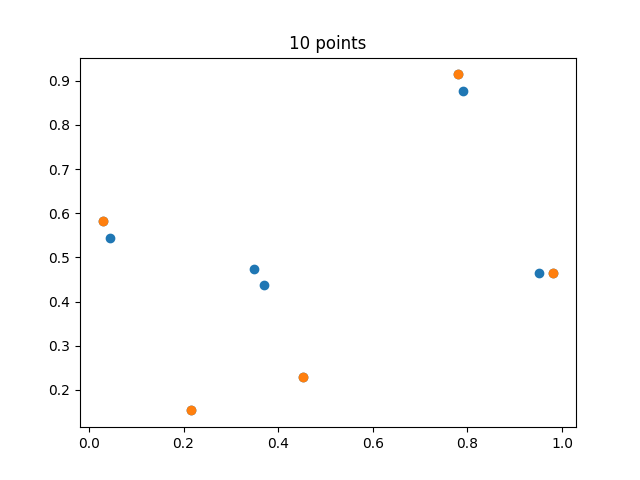
\includegraphics[width=8cm]{10 points.png}
    \caption{10 points, took 0.000015283 seconds to compute.}
\end{figure}
\begin{figure}[h!]
    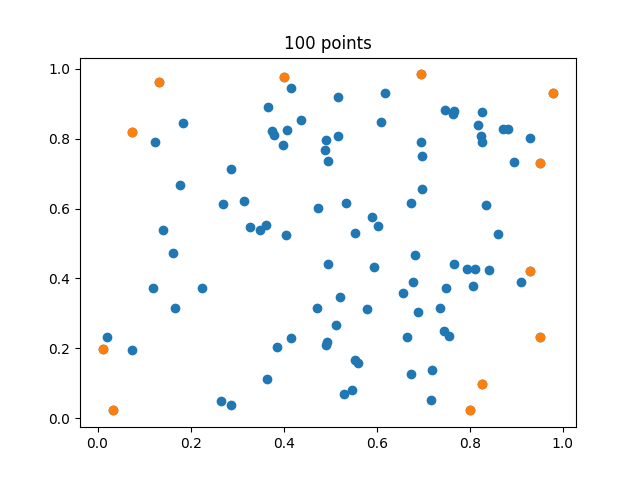
\includegraphics[width=8cm]{100 points.png}
    \caption{100 points, took 0.000027002 seconds to compute.}
\end{figure}
\begin{figure}[h!]
    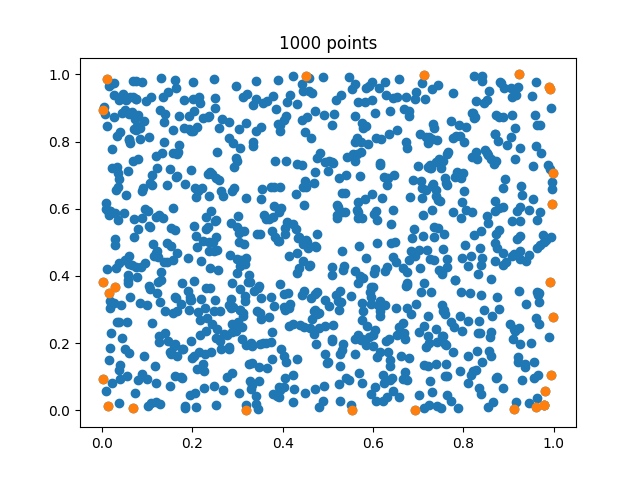
\includegraphics[width=8cm]{1000 points.png}
    \caption{1000 points, took 0.000070175 seconds to compute.}
\end{figure}
\begin{figure}[h!]
    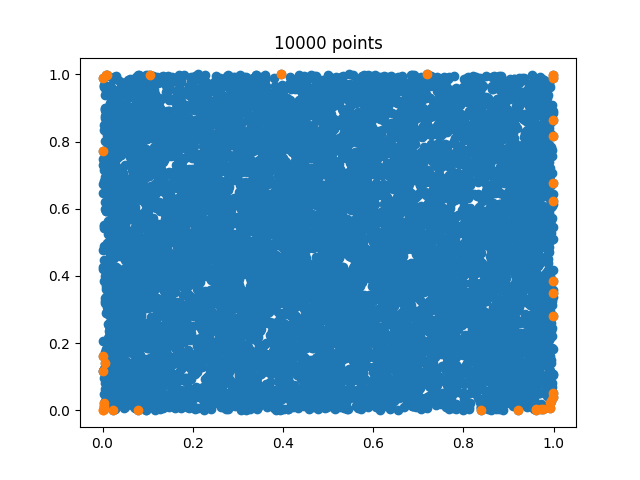
\includegraphics[width=8cm]{10000 points.png}
    \caption{1000 points, took 0.000286934 seconds to compute.}
\end{figure}
\newpage
\begin{lstlisting}
    use nalgebra::Vector2;
use rand::prelude::*;
use serde::Serialize;
use std::{path::Path, time::Instant};
use tokio::{
    fs::File,
    io::{self, AsyncWriteExt},
};
/// gets min along with index of min
fn find_min(points: &[Vector2<f32>]) -> (usize, Vector2<f32>) {
    points.iter().cloned().enumerate().fold(
        (usize::MAX, Vector2::new(f32::MAX, f32::MAX)),
        |acc, x| {
            if x.1.x < acc.1.x {
                x
            } else {
                acc
            }
        },
    )
}
/// gets max along with index of max
fn find_max(points: &[Vector2<f32>]) -> (usize, Vector2<f32>) {
    points.iter().cloned().enumerate().fold(
        (usize::MAX, Vector2::new(f32::MIN, f32::MIN)),
        |acc, x| {
            if x.1.x > acc.1.x {
                x
            } else {
                acc
            }
        },
    )
}
/// splits into two datasets along line with first being above line and second being below line
fn split(
    points: &[Vector2<f32>],
    line_start: Vector2<f32>,
    line_end: Vector2<f32>,
) -> (Vec<Vector2<f32>>, Vec<Vector2<f32>>) {
    let mut upper = vec![];
    let mut lower = vec![];
    for p in points.iter().copied() {
        if is_above(p, line_start, line_end) {
            upper.push(p)
        } else {
            lower.push(p)
        }
    }
    (upper, lower)
}
fn is_above(point: Vector2<f32>, line_start: Vector2<f32>, line_end: Vector2<f32>) -> bool {
    let line = line_end - line_start;
    let point = point - line_start;
    let slope = line.y / line.x;
    let y = point.x * slope;
    y < point.y
}
/// Calculates connvex hull using quick hull
pub fn psudo_hull(points: &mut Vec<Vector2<f32>>) -> Vec<Vector2<f32>> {
    let (min_index, min) = find_min(points);
    let (max_index, max) = find_max(points);

    points.swap_remove(min_index);
    points.swap_remove(max_index);
    let (upper, lower) = split(points, max, min);
    let mut upper_hull = hull_inner(upper, max, min);
    let mut lower_hull = hull_inner(lower, max, min);
    let mut hull = vec![max, min];
    hull.append(&mut upper_hull);
    hull.append(&mut lower_hull);
    hull
}
/// finds firhtest point from line and returns index in array
fn find_furthest(
    points: &[Vector2<f32>],
    line_start: Vector2<f32>,
    line_end: Vector2<f32>,
) -> (usize, Vector2<f32>) {
    let (index, cord, _dist_squared) = points
        .iter()
        .cloned()
        .enumerate()
        .map(|p| {
            let a = p.1 - line_start;
            let line = line_end - line_start;
            (
                p.0,
                p.1,
                a.norm_squared() - (a.dot(&line).powf(2.0) / line.norm_squared()),
            )
        })
        .fold((0, Vector2::new(0.0, 0.0), 0.0), |acc, x| {
            if x.2 > acc.2 {
                x
            } else {
                acc
            }
        });
    (index, cord)
}
/// removes all points lying inside of triangle
fn remove_triangle(points: &mut Vec<Vector2<f32>>, triangle: [Vector2<f32>; 3]) {
    let new_points = points
        .iter()
        .copied()
        .filter(|point| !is_in_triangle(*point, triangle))
        .collect();
    *points = new_points;
}

/// finds out of is in triangle
/// https://stackoverflow.com/questions/2049582/how-to-determine-if-a-point-is-in-a-2d-triangle
fn is_in_triangle(point: Vector2<f32>, triangle: [Vector2<f32>; 3]) -> bool {
    let d1 = sign(point, triangle[0], triangle[1]);
    let d2 = sign(point, triangle[1], triangle[2]);
    let d3 = sign(point, triangle[2], triangle[0]);
    let has_neg = (d1 < 0.0) || (d2 < 0.0) || (d3 < 0.0);
    let has_pos = (d1 > 0.0) || (d2 > 0.0) || (d3 > 0.0);
    !(has_neg && has_pos)
}
fn sign(p1: Vector2<f32>, p2: Vector2<f32>, p3: Vector2<f32>) -> f32 {
    (p1.x - p3.x) * (p2.y - p3.y) - (p2.x - p3.x) * (p1.y - p3.y)
}
fn hull_inner(
    mut points: Vec<Vector2<f32>>,
    line_start: Vector2<f32>,
    line_end: Vector2<f32>,
) -> Vec<Vector2<f32>> {
    if points.is_empty() {
        return vec![];
    }
    let (furthest_index, furthest) = find_furthest(&points, line_start, line_end);
    points.swap_remove(furthest_index);
    let triangle = [line_start, line_end, furthest];
    remove_triangle(&mut points, triangle);
    let (upper, lower) = split(&points, line_start, furthest);
    let mut upper = hull_inner(upper, line_start, furthest);
    let mut lower = hull_inner(lower, furthest, line_end);
    let mut hull = vec![furthest];
    hull.append(&mut upper);
    hull.append(&mut lower);
    hull
}
fn rand_points(n: usize) -> Vec<Vector2<f32>> {
    let mut rng = thread_rng();

    (0..n).map(|_| Vector2::new(rng.gen(), rng.gen())).collect()
}
#[derive(Serialize)]
pub struct PythonVec2 {
    pub x: Vec<f32>,
    pub y: Vec<f32>,
}

impl From<&Vec<Vector2<f32>>> for PythonVec2 {
    fn from(data: &Vec<Vector2<f32>>) -> Self {
        let mut x = vec![];
        let mut y = vec![];
        for v in data.iter() {
            x.push(v.x);
            y.push(v.y);
        }
        Self { x, y }
    }
}
#[derive(Serialize)]
pub struct HullResult {
    points: PythonVec2,
    hull: PythonVec2,
    time_s: f32,
}
async fn run_hull<P: AsRef<Path>>(n: usize, path: P) -> io::Result<()> {
    let mut points = rand_points(n);
    let out_points: PythonVec2 = (&points).into();
    let now = Instant::now();

    let hull = psudo_hull(&mut points);
    let time_s = now.elapsed().as_secs_f32();
    let result = HullResult {
        points: out_points,
        hull: (&hull).into(),
        time_s,
    };
    let mut f = File::create(path).await?;
    let hull_data = serde_json::to_string_pretty(&result).expect("failed to parse");
    f.write_all(hull_data.as_bytes()).await?;

    Ok(())
}
/// NOTE TO FUTURE ME READ THIS
///https://steamcdn-a.akamaihd.net/apps/valve/2014/DirkGregorius_ImplementingQuickHull.pdf
#[tokio::main]
async fn main() -> io::Result<()> {
    run_hull(10, "10.json").await?;
    run_hull(100, "100.json").await?;
    run_hull(1000, "1000.json").await?;
    run_hull(10000, "10000.json").await?;
    Ok(())
}
#[cfg(test)]
mod test {
    use super::*;
    #[test]
    fn min() {
        let points = [
            Vector2::new(0.0, 0.0),
            Vector2::new(1.0, 0.0),
            Vector2::new(0.5, 1.0),
        ];
        let min = find_min(&points);
        assert_eq!(min, (0, Vector2::new(0.0, 0.0)));
    }
    #[test]
    fn max() {
        let points = [
            Vector2::new(0.0, 0.0),
            Vector2::new(1.0, 0.0),
            Vector2::new(0.5, 1.0),
        ];
        let min = find_max(&points);
        assert_eq!(min, (1, Vector2::new(1.0, 0.0)));
    }
    #[test]
    fn basic() {
        let triangle = [
            Vector2::new(0.0, 0.0),
            Vector2::new(1.0, 0.0),
            Vector2::new(0.5, 1.0),
        ];
        assert_eq!(is_in_triangle(Vector2::new(0.5, 0.25), triangle), true);
        assert_eq!(is_in_triangle(Vector2::new(1.5, 0.25), triangle), false);
        assert_eq!(is_in_triangle(Vector2::new(0.5, 1.25), triangle), false);
    }
}
\end{lstlisting}
code:
\url{https://github.com/scifi6546/cs411_cards}

\end{document}
